\subsection{Experiment 1: General Applicability}

The training of the model took approximately 11 days until convergence. 
Training stopped at $6.7\cdot10^5$ due to no improvement in gamma and validation loss. 
The model reaches mean gamma passrates of 94.35\% ± 5.99\% (min: 58.02\%, max: 99.96\%) for prostate test segments and a mean gamma passrate of 99.1\% ± 1.3\% (min: 96.8\%, max: 100\%) for the five plans.
Very good dose agreement between target dose, caluclated \acs{MC} simulation and the dose prediction can be observed as depicted in \autoref{fig:prediction}, showing the isocentric slice of a prostate cancer patient with a gamma passrate of 99.9\%.
As shown, the model is able to accurately predict the beamshape for single segments as well as the penumbra and beamwidening. 
The \ac{DVH} shown in \autoref{fig:dvh} gives crucial information about the applied dose inside target volumes as well as \ac{OAR} for a test plan of the prostate patient cohort.
\acs{DVH} curves overlap for all structures but urethra, which was caused by the high contribution of single voxels to the entire volume. 
Very good dose agreement for high as well as low dose regions was reached. 

\begin{figure}[htb]
    \centering
    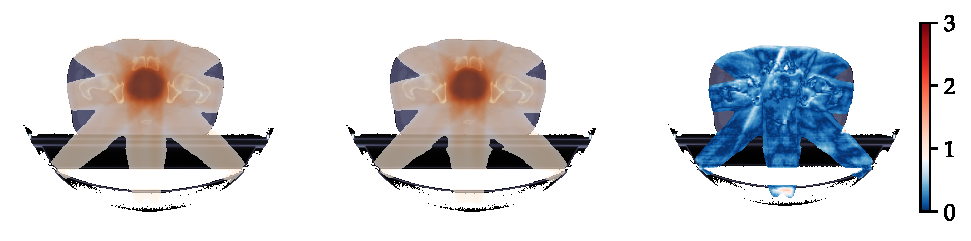
\includegraphics[width=\textwidth]{gamma_pt0.pdf}
    \caption{
        Dose prediction example on isocentric slice on prostate cancer patient from test cohort with prostate data only trained model. 
        From left to right: target dose; dose prediction; gamma map for isocentric slice with a gamma pass rate of 99.9\%
    }\label{fig:prediction}
\end{figure}

\begin{figure}
    \centering
    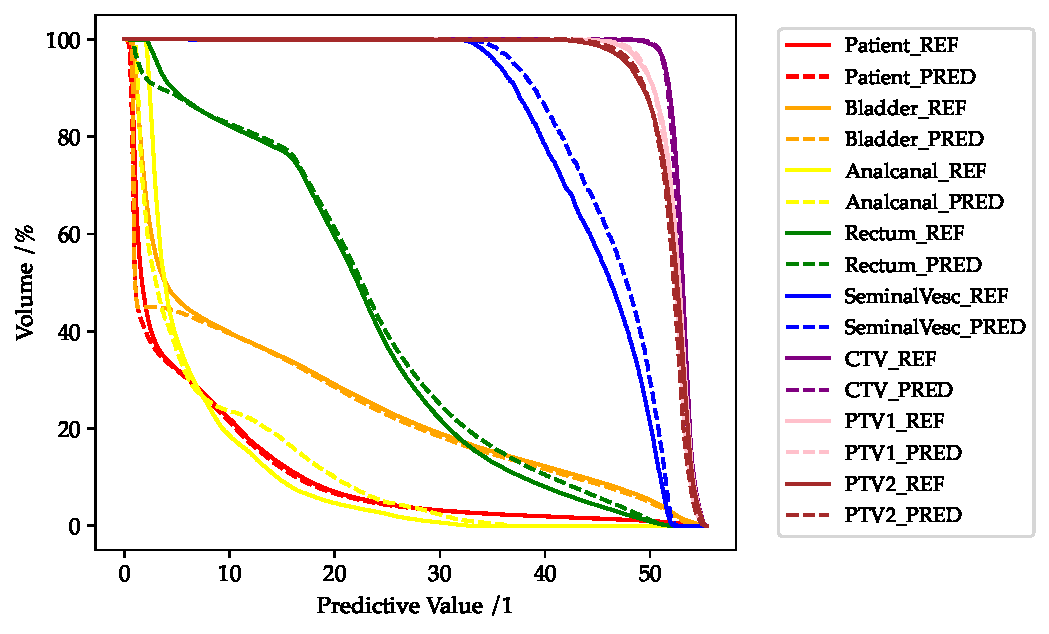
\includegraphics[scale=0.7]{dvh.pdf}
    \caption{\acs{DVH} for prostate cancer test plan with gamma passrate of 99.9\%.}\label{fig:dvh}
\end{figure}

\subsection{Experiment 2: Poor Initial Translatability}

When applying the prostate only trained network on body entities deviating from the lower abdomen its accuracy decreases significantly. 
A summary over the prediction accuracy for all segments as well as the summed plans for all included test data of different entities is given in \autoref{tab:prost}. 

\begin{table}[htb]
    \centering
    \scalebox{1}{
        \begin{tabular}{|lccccccccccc|}
            \hline
            \multicolumn{1}{|r}{}              & \multicolumn{1}{l}{} & \multicolumn{2}{c}{\textbf{Prostate}} & \multicolumn{2}{c}{\textbf{Liver}} & \multicolumn{2}{c}{\textbf{Mamma}} & \multicolumn{2}{c}{\textbf{H\&N}} & \multicolumn{2}{c|}{\textbf{LN}} \\
            \multirow{2}{*}{} & \multirow{2}{*}{\#}  & \textit{Seg.}     & \textit{Plans}     & \textit{Seg.}    & \textit{Plans}   & \textit{Seg.}    & \textit{Plans}   & \textit{Seg.}   & \textit{Plans}   & \textit{Seg.}   & \textit{Plans}  \\
                                               &                      & 306               & 5                 & 272              & 5               & 419              & 5               & 379             & 5               & 659             & 15             \\ \hline
            \textbf{Mean}                      & \multirow{5}{*}{/\%}  & 94.3              & \textbf{99.1}              & 75.4             & 89.9            & 57.8             & 67.4            & 60.5            & 77.4            & 77.4            & 93.0           \\
            \textbf{Median}                    &                      & \textbf{96.2}              & \textbf{99.6}              & 77.4             & 91.8            & 56.4             & 66.2            & 61.0            & 78.8            & 80.2            & 92.8           \\
            \textbf{STD}                       &                      & 6.0               & 1.3               & 12.6             & 4.1             & 18.0             & 5.3             & 11.8            & 10.2            & 13.8            & 6.1            \\
            \textbf{Min}                       &                      & 58.0              & 96.8              & 38.9             & 84.0            & 1.9              & 60.6            & 31.1            & 62.5            & 36.0            & 75.3           \\
            \textbf{Max}                       &                      & 100               & 99.9              & 99.4             & 94.4            & 94.7             & 73.0            & 91.5            & 90.2            & 99.7            & 99.7           \\ \hline
            \end{tabular}}
    \caption{Gamma rassrates for segments as well as plans for prostate, liver, mamma, \acs{HN} and \acs{LN} predicted with the prostate-only trained model. Gamma test settings: 3~mm/3\% lower percentage cutoff 10\%}\label{tab:prost}
\end{table}

The model shows particular problems with breast cancer and \acs{HN} segments with a mean gamma passrate of 57.8~±~18.0\% (min: 1.9\% max: 94.7\%) and 60.5~±~11.8\% (min: 31.1\% max: 91.5\%). 
An examplary case with a gamma passrate of 60.6\% is shown in \autoref{fig:mamma_pred} depicting low accuracy in the high dose as well as lower dose areas of the volume.


\begin{figure}
    \centering
    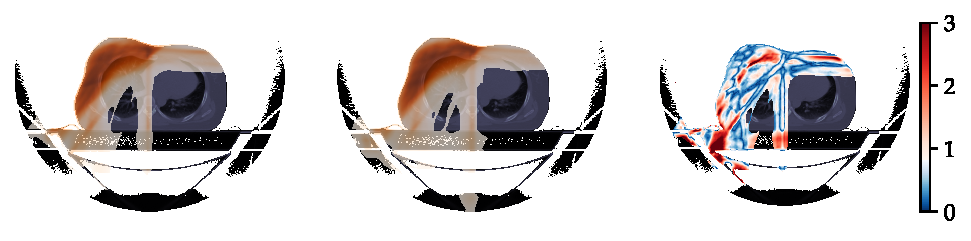
\includegraphics[width=\textwidth]{gamma_mt1.pdf}
    \caption{
        Dose prediction example on isocentric slice on breast cancer patient from test cohort with prostate data only trained model. 
        From left to right: target dose; dose prediction; gamma map for respective slice with a gamma pass rate of 60.6\%}\label{fig:mamma_pred}
\end{figure}

\subsection{Experiment 3: Increased Robustness}

The model training took approximately 9 days until convergence. Training stopped after $5.0\cdot10^7$ patches due to no improvement in gamma and validation loss. 
Testing was done on prostate, liver, mamma and \acs{HN} plans, which were contained in the training set as well as \acs{LN} plans which were not included. 
A summary of the reached gamma passrates is given in \autoref{tab:mixed}, showing significantly improved gamma passrates with respect to \emph{Experiment 2}, see \autoref{fig:comparison}~\emph{left}.
Mean gamma pass rate for single segments changed by -0.88\%, +14.4\%, +19.11\%, +19.65\%, +7.75\% for prostate, liver, mamma, \acs{HN} and \acs{LN} respectively. 
The mean gamma passrate shows increased performance for the plan analysis of all tumor entities with an increase of  +0.1\%,  +7.7\%,+16.2\%, +11.4\%, +3\% for prostate, liver, mamma, \acs{HN} and \acs{LN} plans respectively. 
A comparison between the results of the individual segments and the overall plans showed that, on average, the segments with the higher contributions to the dose distribution of the entire plan were better predicted than less contributing ones. 

\begin{table}[!htb]
    \centering
    \scalebox{1}{
        \begin{tabular}{|lccccccccccc|}
            \hline
            \multicolumn{1}{|r}{}              & \multicolumn{1}{l}{} & \multicolumn{2}{c}{\textbf{Prostate}} & \multicolumn{2}{c}{\textbf{Liver}} & \multicolumn{2}{c}{\textbf{Mamma}} & \multicolumn{2}{c}{\textbf{H\&N}} & \multicolumn{2}{c|}{\textbf{LN}} \\
            \multirow{2}{*}{} & \multirow{2}{*}{\#}  & \textit{Seg.}     & \textit{Plans}     & \textit{Seg.}    & \textit{Plans}   & \textit{Seg.}    & \textit{Plans}   & \textit{Seg.}   & \textit{Plans}   & \textit{Seg.}   & \textit{Plans}  \\
                                               &                      & 306               & 5                 & 272              & 5               & 419              & 5               & 379             & 5               & 659             & 15             \\ \hline
            \textbf{Mean}                      & \multirow{5}{*}{/\%}  & 93.5              & \textbf{99.2}              & 89.8             & \textbf{97.6}            & 76.9             & 83.6            & 80.1            & 88.8            & 85.2            & \textbf{96.0}          \\
            \textbf{Median}                    &                      & \textbf{95.0}              & \textbf{99.7}              & 91.6             & \textbf{97.4}            & 78.9             & 83.7            & 82.8            & 90.9            & 87.8            & \textbf{98.8}           \\
            \textbf{STD}                       &                      & 6.3               & 1.0               & 7.0              & 1.0             & 12.8             & 4.6             & 10.9            & 8.6             & 10.7            & 5.8            \\
            \textbf{Min}                       &                      & 39.2              & 97.5              & 50.8             & 96.6            & 18.4             & 77.0            & 49.3            & 76.0            & 38.7            & 77.9           \\
            \textbf{Max}                       &                      & 99.8              & 99.9              & 99.1             & 99.2            & 98.5             & 89.8            & 97.4            & 98.5            & 99.9            & 99.9           \\ \hline
            \end{tabular}}
    \caption{Gamma rassrates for segments as well as plans for prostate, liver, mamma, \acs{HN} and \acs{LN} predicted with the mixed data trained model. Gamma test settings: 3~mm/3\% lower percentage cutoff 10\%}\label{tab:mixed}
\end{table}

To get a deeper insight into the networks method of operation and to enlarge the interpretability of the network, we analysed the perfomance of the network regarding field size and segment weights as depicted in \autoref{fig:weight_fz_analysis}, which gives information about the correlation of field size and prediction accuracy of single segments. 
Relative occurence of segment sizes as well as weights are displayed as a bar chart in the background of both plots.
Around 82\% of all segments have a field size smaller than 60~cm\textsuperscript{2} that is also the field size until network accuracy increases with increasing field size for both the prostate-only and mixed entity trained model.
Field sizes larger than 60~cm\textsuperscript{2} are not predicted as stable with fluctuating gamma passrates for both models.
The prostate-only trained model experienced a larger drop in accuracy for field sizes larger than 60~cm\textsuperscript{2} and accuracy is steadily decreasing with increasing field sizes. 
It was observable that smaller field sizes are less robust and range from 1.9\% to 100\% and 18.5\% to 99.9\% for the prostate-only and the mixed entity model respectively on a field size of 0 to 15~cm\textsuperscript{2}.
Gamma passrate analysis with respect to segment weight showed the same trend of increased accuracy and robustness with increasing weight values.
Segments with weights under 0.2 made up for almost 80\% of all segments. 
A comprehensive and direct comparison between prostate-only and mixed entity model prediction accuracy for segment and plan predictions is given in \autoref{tab:seg_comp} and \autoref{tab:plan_comp}.

\begin{figure}[htb]
    \centering
    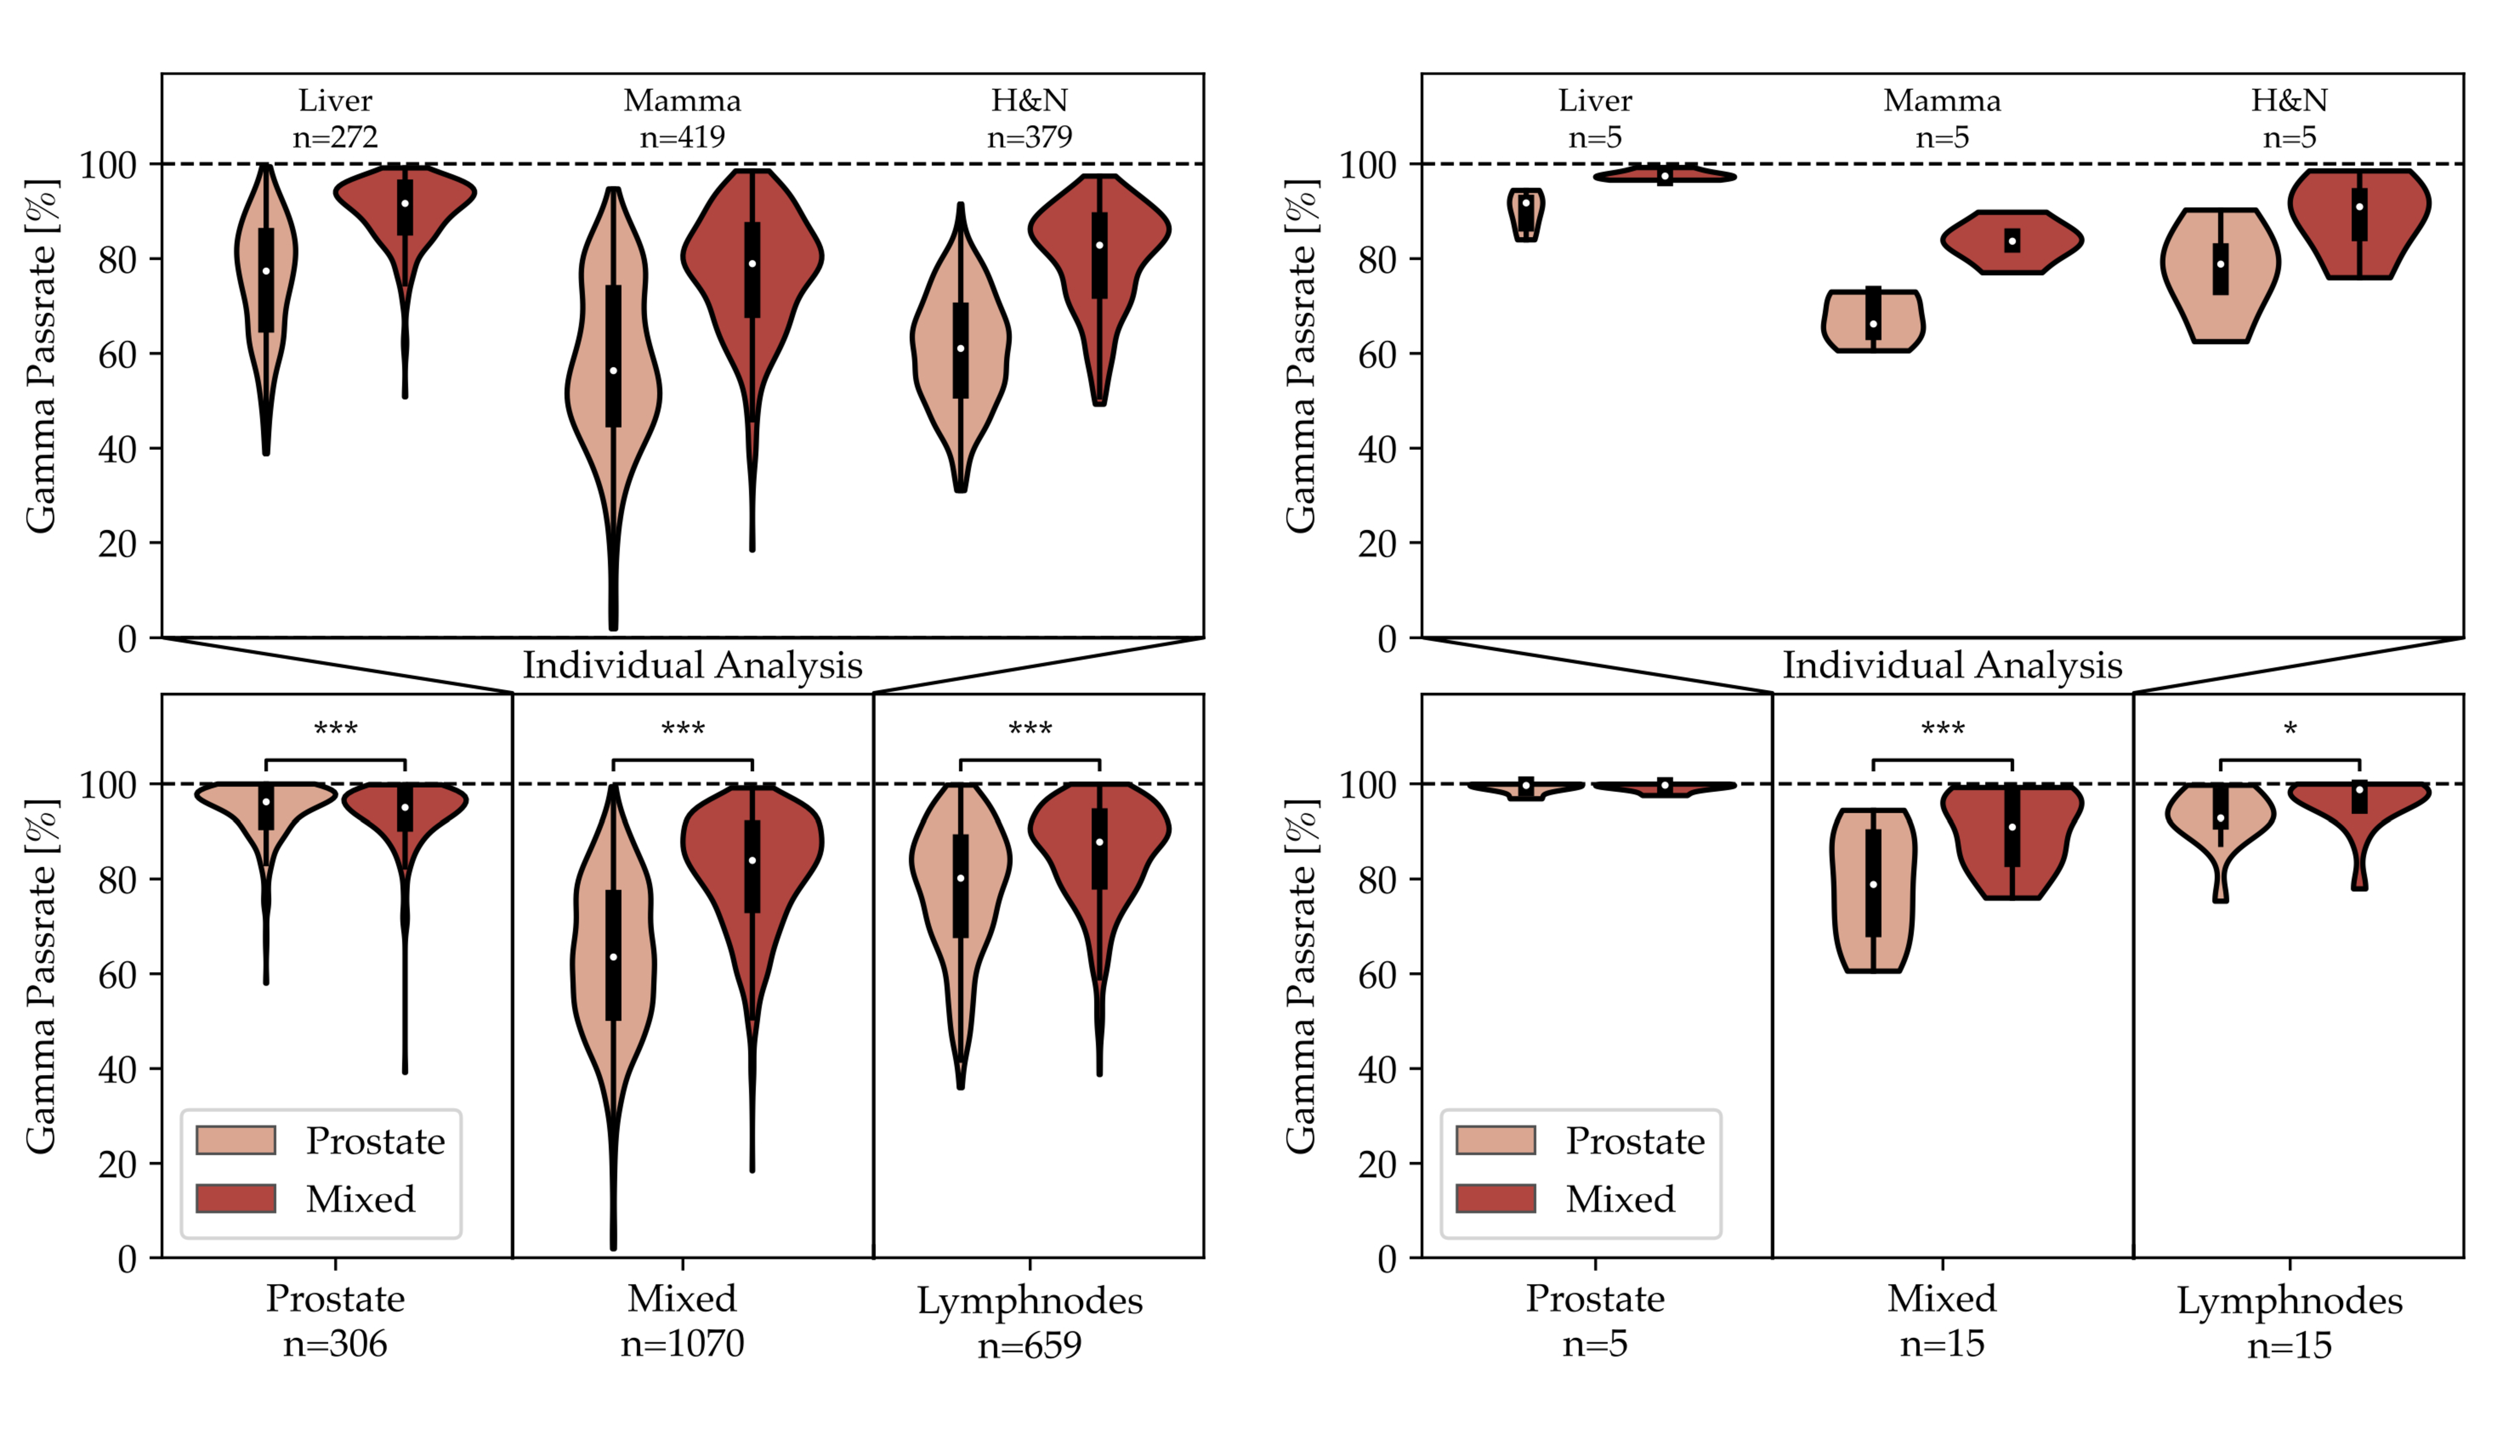
\includegraphics[width=\textwidth]{results_combined.pdf}
    \caption{
        Gamma pass rate comparison for single segments (left) and summed up plans (right) between prostate-only and mixed entity trained models. 
        Boxplot are displayed inside respecitve violin plots. 
        Individual analysis of the mixed entity set, composed of liver, mamma and \acs{HN} is displayed on top plot. 
        Significance level was assessed using Wilcoxon singed-rank test with significance level p~<~0.05~(*), p~<~0.01~(**) and p~<~0.001~(***).
    }\label{fig:comparison}
\end{figure}

\newpage

\begin{figure}[!h]
    \centering
    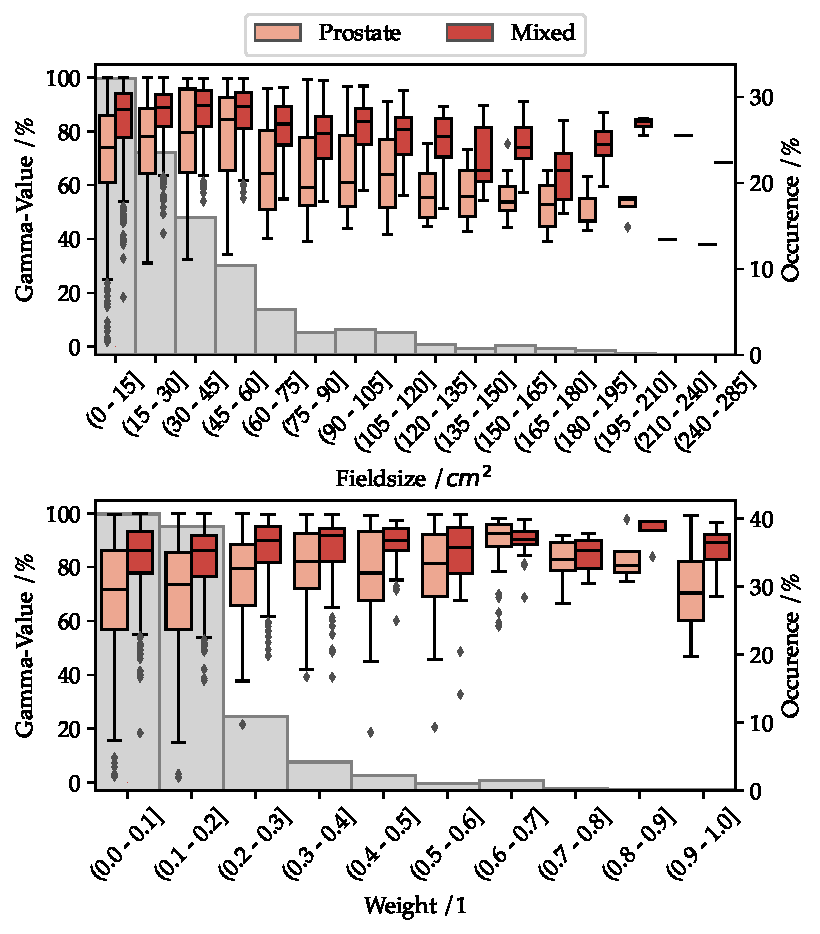
\includegraphics[width=\textwidth]{segs_weight_fz.pdf}
    \caption{
        Prediction accuracy of each segment with respect to field size for prostate only and mixed trained model. 
        Relative occurence of discretized field size bin is displayed in the background.}\label{fig:weight_fz_analysis}
\end{figure}

\newpage

\begin{table}[htb]
    \centering
    \scalebox{0.78}{
        \begin{tabular}{|llcccccccccc|}
            \hline
            \multicolumn{1}{|r}{} &                     & \multicolumn{2}{c}{\textbf{Prostate}} & \multicolumn{2}{c}{\textbf{Liver}} & \multicolumn{2}{c}{\textbf{Mamma}} & \multicolumn{2}{c}{\textbf{H\&N}}  & \multicolumn{2}{c|}{\textbf{LN}}   \\
            \textbf{Model}        &                     & \textit{Prostate}   & \textit{Mixed}  & \textit{Prostate} & \textit{Mixed} & \textit{Prostate} & \textit{Mixed} & \textit{Prostate} & \textit{Mixed} & \textit{Prostate} & \textit{Mixed} \\ \hline
            \textbf{Mean}         & \multirow{5}{*}{/\%} & 94.3                & 93.5            & 75.4              & 89.8           & 57.8              & 76.9           & 60.5              & 80.1           & 77.4              & 85.2           \\
            \textbf{Median}       &                     & \textbf{96.2}                & \textbf{95.0}            & 77.4              & 91.6           & 56.4              & 78.9           & 61.0              & 82.8           & 80.2              & 87.8           \\
            \textbf{STD}          &                     & 6.0                 & 6.3             & 12.6              & 7.0            & 18.0              & 12.8           & 11.8              & 10.9           & 13.8              & 10.7           \\
            \textbf{Min}          &                     & 58.0                & 39.2            & 38.9              & 50.8           & 1.9               & 18.4           & 31.1              & 49.3           & 36.0              & 38.7           \\
            \textbf{Max}          &                     & 100.0               & 99.8            & 99.4              & 99.1           & 94.7              & 98.5           & 91.5              & 97.4           & 99.7              & 99.9           \\ \hline
        \end{tabular}
        }
    \caption{Gamma passrate comparison of prostate-only and mixed entity trained models on the test dataset consisting of 306 prostate, 272 liver, 419 mamma, 379 head \& neck and 659 lymphnode segments. Gamma test criteria: 3~mm/3\% with a lower dose cutoff of 10\%.}\label{tab:seg_comp}
    \end{table}


\begin{table}[htb]
    \centering
    \scalebox{0.78}{
        \begin{tabular}{|lccccccccccc|}
            \hline
            \multicolumn{1}{|r}{} & \multicolumn{1}{l}{} & \multicolumn{2}{c}{\textbf{Prostate}} & \multicolumn{2}{c}{\textbf{Liver}} & \multicolumn{2}{c}{\textbf{Mamma}} & \multicolumn{2}{c}{\textbf{H\&N}}  & \multicolumn{2}{c|}{\textbf{LN}}   \\
            \textbf{Model}        & \multicolumn{1}{l}{} & \textit{Prostate}   & \textit{Mixed}  & \textit{Prostate} & \textit{Mixed} & \textit{Prostate} & \textit{Mixed} & \textit{Prostate} & \textit{Mixed} & \textit{Prostate} & \textit{Mixed} \\ \hline
            \textbf{Mean}         & \multirow{5}{*}{/\%}  & \textbf{99.1}                & \textbf{99.2}            & 89.9              & \textbf{97.6}           & 67.4              & 83.6           & 77.4              & 88.8           & 93.0              & \textbf{96.0}           \\
            \textbf{Median}       &                      & \textbf{99.6}                & \textbf{99.7}            & 91.8              & \textbf{97.4}           & 66.2              & 83.7           & 78.8              & 90.9           & 92.8              & \textbf{98.8}           \\
            \textbf{STD}          &                      & 1.3                 & 1.0             & 4.1               & 1.0            & 5.3               & 4.6            & 10.2              & 8.6            & 6.1               & 5.8            \\
            \textbf{Min}          &                      & 96.8                & 97.5            & 84.0              & 96.6           & 60.6              & 77.0           & 62.5              & 76.0           & 75.3              & 77.9           \\
            \textbf{Max}          &                      & 99.9                & 99.9            & 94.4              & 99.2           & 73.0              & 89.8           & 90.2              & 98.5           & 99.7              & 99.9           \\ \hline
            \end{tabular}
        }
    \caption{{Gamma passrate comparison of prostate-only and mixed entity trained models on the test dataset consisting of 5 prostate, 5 liver, 5 mamma, 5 head \& neck and 15 lymphnode treatment plans. Gamma test criteria: 3~mm/3\% with a lower dose cutoff of 10\%.}}\label{tab:plan_comp}
\end{table}

\subsection{Experiment 4: Underlying Physics}

Both the prostate-only as well as the mixed entity model perform poorly regarding gamma passrates for all water phantom positions tested. 
The model accuracy is steadily decreasing with increasing \acs{SSD} and gamma pass rates of 60.1\%, 45.5\%, 48.4\%, and 56.1\%, 27.7\%, 19.2\% for the prostate-only and mixed entity model at depths of 100~pixels, 200~pixels and 300~pixels respectively. A summary of the accuracy is given in \autoref{tab:phantom_res}. 
The transversal view in \autoref{fig:phantom} shows that the prostate model is better at representing the peak at the beginning of the phantom than the mixed model for a depth of 100 pixels. 
At higher phantom distances the prostate model resembles the qualitative dose distribution quite well while failing at achieving a quantitatively correct predictive value. 
The mixed model cannot reach the correct peak height at the beginning but predicts the later curve very well in terms of height and curvature in the transversal view. 
Coronal and sagittal view both show that the penumbra is resembled very well by both models. 
At phantom depths of 200 and 300 pixels the shoulders of the dose profile drop too fast for the mixed trained model in the coronal view.
Slight fluctuations at the phantom's edge can be observed at 100~pixel depth for the mixed model in the sagittal view.
 
\begin{table}
    \begin{tabular}{|lc|cc|cc|cc|}
    \hline
    Phantom position & /pixel & \multicolumn{2}{c|}{\textbf{100}} & \multicolumn{2}{c|}{\textbf{200}} & \multicolumn{2}{c|}{\textbf{300}} \\ \hline
    Model               &        & Mixed          & Prostate         & Mixed          & Prostate         & Mixed          & Prostate         \\
    Gamma Passrate      & /\%    & 60.1         & 56.1           & 45.5         & 27.7           & 48.4         & 19.2           \\ \hline
    \end{tabular}
    \caption{Gamma passrates for prostate only and mixed trained models for different water phantom positions inside an air volume. Water phantom thickness was 200 pixels.}\label{tab:phantom_res}
\end{table}

\begin{figure}[htb]
    \centering
    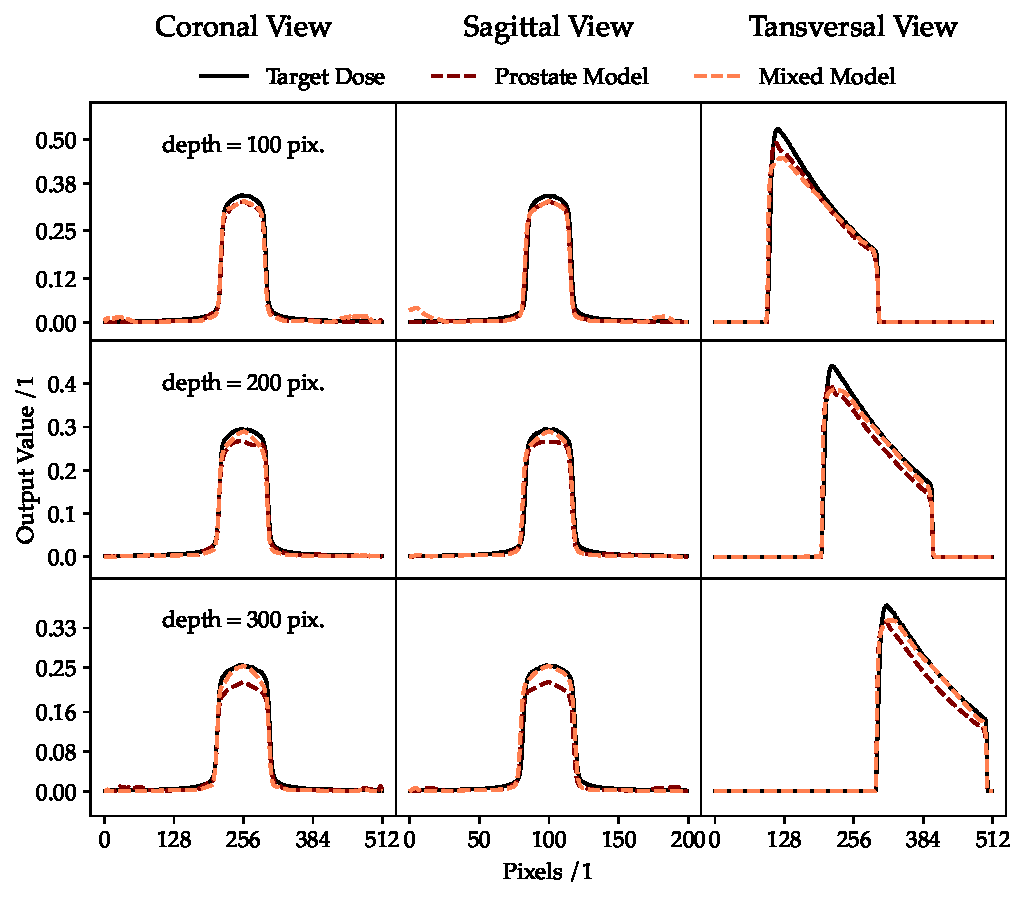
\includegraphics[width=0.8\textwidth]{quer.pdf}
    \caption{Coronal, sagital and transversal view of the dose distributions for 100, 200 and 300 px depth in the phantom volume.}\label{fig:phantom}
\end{figure}